\documentclass[11pt]{article}

\usepackage[T1]{fontenc}
\usepackage{lmodern}
\usepackage[margin=0.90in]{geometry}
\usepackage{microtype}
\usepackage{amsmath,amssymb,amsthm,mathtools}
\usepackage{booktabs,longtable,array,tabularx}
\usepackage{graphicx}
\usepackage{float}
\usepackage{xcolor}
\usepackage{enumitem}
\usepackage{fancyhdr}
\usepackage{hyperref}
\usepackage[nameinlink,noabbrev]{cleveref}
\usepackage{listings}
\usepackage{caption}
\usepackage{bm}
\usepackage{needspace}
\usepackage{placeins}

\graphicspath{{figures/}}
\allowdisplaybreaks

\hypersetup{
  pdftitle={Projector-Resolved Seed Calculus VII},
  pdfauthor={Komorebi P.},
  pdfsubject={Quantum seeds, symmetry packets, circuit paths, effective dynamics, quantum channels, geometric connections, and quantum-spacetime refinement},
  colorlinks=true,
  linkcolor=black,
  citecolor=black,
  urlcolor=black
}

\pagestyle{fancy}
\fancyhf{}
\fancyhead[L]{Projector-Resolved Seed Calculus VII}
\fancyhead[R]{Komorebi P.}
\fancyfoot[C]{\thepage}
\setlength{\headheight}{14pt}

\newtheorem{theorem}{Theorem}[section]
\newtheorem{proposition}[theorem]{Proposition}
\newtheorem{lemma}[theorem]{Lemma}
\newtheorem{corollary}[theorem]{Corollary}
\theoremstyle{definition}
\newtheorem{definition}[theorem]{Definition}
\newtheorem{example}[theorem]{Example}
\newtheorem{construction}[theorem]{Construction}
\newtheorem{conjecture}[theorem]{Conjecture}
\theoremstyle{remark}
\newtheorem{remark}[theorem]{Remark}
\newtheorem{boundary}[theorem]{Boundary}
\newtheorem{certificate}[theorem]{Numerical Certificate}
\newtheorem{classical}[theorem]{Classical Input}

\newcommand{\cA}{\mathcal A}
\newcommand{\cB}{\mathcal B}
\newcommand{\cC}{\mathcal C}
\newcommand{\cE}{\mathcal E}
\newcommand{\cF}{\mathcal F}
\newcommand{\cG}{\mathcal G}
\newcommand{\cH}{\mathcal H}
\newcommand{\cK}{\mathcal K}
\newcommand{\cL}{\mathcal L}
\newcommand{\cO}{\mathcal O}
\newcommand{\cD}{\mathcal D}
\newcommand{\cP}{\mathcal P}
\newcommand{\cR}{\mathcal R}
\newcommand{\cS}{\mathcal S}
\newcommand{\cT}{\mathcal T}
\newcommand{\bbC}{\mathbb C}
\newcommand{\bbR}{\mathbb R}
\newcommand{\bbZ}{\mathbb Z}
\newcommand{\bbN}{\mathbb N}
\newcommand{\Id}{\operatorname{Id}}
\newcommand{\Tr}{\operatorname{Tr}}
\newcommand{\rank}{\operatorname{rank}}
\newcommand{\Ran}{\operatorname{Ran}}
\newcommand{\Ker}{\operatorname{Ker}}
\newcommand{\Spec}{\operatorname{Spec}}
\newcommand{\diag}{\operatorname{diag}}
\newcommand{\ad}{\operatorname{ad}}
\newcommand{\norm}[1]{\left\lVert#1\right\rVert}
\newcommand{\ket}[1]{\left|#1\right\rangle}
\newcommand{\bra}[1]{\left\langle#1\right|}
\newcolumntype{L}[1]{>{\raggedright\arraybackslash}p{#1}}
\newcolumntype{Y}{>{\raggedright\arraybackslash}X}

\lstset{
  language=Python,
  basicstyle=\ttfamily\footnotesize,
  breaklines=true,
  frame=single,
  showstringspaces=false,
  columns=fullflexible,
  keepspaces=true,
  numbers=left,
  numberstyle=\tiny,
  numbersep=7pt
}

\title{\textbf{Projector-Resolved Seed Calculus VII}\\[0.45em]
\large Quantum Seed Calculus: Symmetry Packets, Circuits, Effective Dynamics, and Quantum Spacetime}
\author{Komorebi P.}
\date{}

\begin{document}
\maketitle

\begin{abstract}
This paper develops the finite quantum realization of the projector-resolved seed calculus. A quantum seed is propagated by a declared gate or observable grammar, resolved into symmetry packets, transferred through circuit paths, and reconstructed exactly. For finite observable algebras, the dimension of the orbit generated by a seed is computed from the ranks of its multiplicity matrices, yielding an explicit quantum seed-rank formula. Cyclic symmetry projectors and tensor/polyphase refinement are proved in a common operator language. Quantum circuits admit an exact path expansion over intermediate packet addresses, and unitarity becomes a packetwise conservation law. For Hamiltonian evolution, exact symmetry produces invariant packets, while a Duhamel argument bounds leakage by the commutator with the packet projector. Moving coordinate frames require a connection term; a canonical skew-Hermitian projector connection is constructed and shown to transport the complete packet family. The curvature of a projector bundle is expressed as $P(dP\wedge dP)P$, with the Bloch-sphere line bundle as a worked example. Measurements and completely positive maps are resolved into packet superoperators, and the Knill--Laflamme condition is interpreted as annihilation of the code obstruction packet. Exact Schur--Feshbach reduction proves that hidden sectors return as a spectral self-energy and, in time coordinates, as a memory kernel. The final sections formulate a finite projector geometry for quantum spacetime, prove positivity and composition of Euclidean transfer operators, test one- and two-dimensional spectral dimensions, and isolate the continuum, constraint, Lorentzian, Einstein-limit, and spin-two statements that remain conjectural. Nineteen code-generated figures, machine-readable results, and twenty-two automated tests accompany the paper. Finite theorems, classical inputs, numerical certificates, and conjectural physical claims are kept separate.
\end{abstract}

\begin{center}
\fbox{\begin{minipage}{0.93\textwidth}
\textbf{Scope and claim boundary.} The paper proves the stated finite-dimensional results concerning quantum seed rank, exact packet reconstruction, cyclic symmetry projectors, tensor refinement, circuit path expansion, packet unitarity, leakage bounds, moving frames, projector connections, rank-one curvature, Kraus channels, block-diagonal measurement invariance, the finite Knill--Laflamme criterion, Schur--Feshbach reduction, and finite spectral diagnostics. It does not claim a solution of quantum gravity, a construction of an interacting continuum quantum field theory, anomaly-free gravitational constraints, Lorentzian reconstruction, the Einstein infrared limit, or the existence of a physical massless spin-two sector. Classical references are reserved for the consolidated end-of-series bibliography and are not reproduced here.
\end{minipage}}
\end{center}

\tableofcontents
\listoffigures
\listoftables
\clearpage

\section{The quantum seed realization}

The common operator sequence of the series becomes
\[
\boxed{
\begin{gathered}
\text{quantum seed}
\longrightarrow
\text{gate or observable address}
\longrightarrow
\text{symmetry projection}\\
\longrightarrow
\text{packet transfer}
\longrightarrow
\text{constraint}
\longrightarrow
\text{refinement}
\longrightarrow
\text{reconstruction}
\end{gathered}
}
\]

\begin{figure}[htbp]
\centering
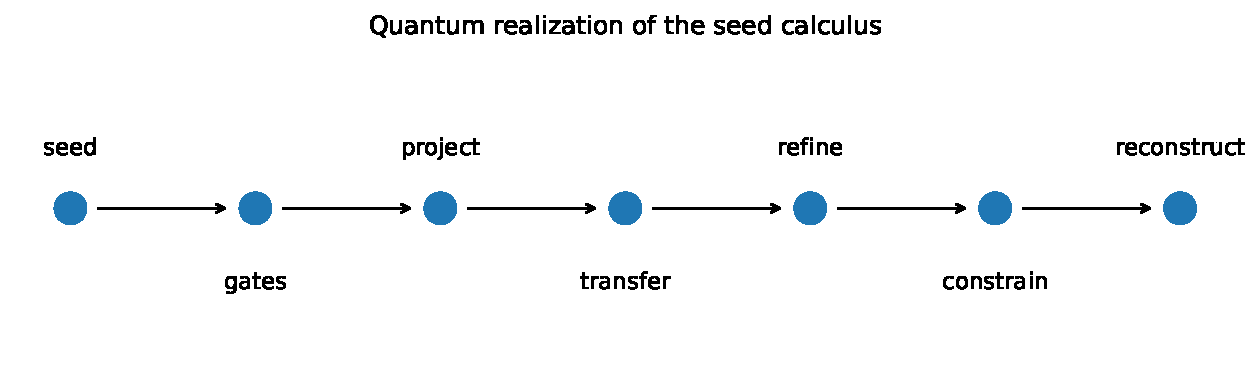
\includegraphics[width=0.98\textwidth]{01_quantum_seed_architecture.pdf}
\caption{The quantum realization of the common seed-calculus operator chain. The same finite packet language is used for states, gates, Hamiltonians, channels, geometric projectors, and effective dynamics.}
\label{fig:architecture}
\end{figure}

\begin{definition}[Finite quantum seed system]
A finite quantum seed system is a tuple
\[
\mathfrak Q=
\left(
\cH,
\psi_0,
\cO,
\cR,
\{P_{\ell,\alpha}\},
H,
\tau
\right),
\]
where $\cH$ is a finite-dimensional Hilbert space, $\psi_0\in\cH$ is a nonzero seed, $\cO$ is the declared operator grammar, $\cR$ is a collection of algebraic or physical constraints, $\{P_{\ell,\alpha}\}$ is an exact packet system at each refinement level, $H=H^*$ is a Hamiltonian when dynamics are present, and $\tau$ specifies the topology used in a later completion.
\end{definition}

The generated state space is
\[
\cH(\psi_0;\cO)
=
\operatorname{span}
\left\{
O_r\cdots O_1\psi_0:
O_j\in\cO,
\ r\ge0
\right\}.
\]
The quantum seed is cyclic for the grammar when
\[
\cH(\psi_0;\cO)=\cH.
\]
This is a statement about the pair $(\psi_0,\cO)$, not about the vector alone. A state may be cyclic for the full matrix algebra and noncyclic for a restricted physical gate set.

\section{Quantum seed rank and cyclicity}

\subsection{Finite observable algebras}

Let a finite-dimensional $*$-algebra act in its standard multiplicity form
\[
\cA
\cong
\bigoplus_{i=1}^r
\left(M_{d_i}(\bbC)\otimes I_{m_i}\right)
\]
on
\[
\cH
\cong
\bigoplus_{i=1}^r
\left(\bbC^{d_i}\otimes\bbC^{m_i}\right).
\]
A vector $\psi_i\in\bbC^{d_i}\otimes\bbC^{m_i}$ is identified with a $d_i\times m_i$ coefficient matrix $C_i$.

\begin{theorem}[Orbit dimension of one quantum seed]
For the action of $M_d(\bbC)\otimes I_m$ on $\bbC^d\otimes\bbC^m$, let $C$ be the coefficient matrix of a seed $\psi$. Then
\[
\boxed{
\dim\operatorname{span}\{(A\otimes I_m)\psi:A\in M_d(\bbC)\}
=d\,\rank C.
}
\]
The seed is cyclic if and only if $\rank C=m$, which is possible only when $m\le d$.
\end{theorem}

\begin{proof}
Under the coefficient-matrix identification, $(A\otimes I_m)\psi$ corresponds to $AC$. Every row of $AC$ lies in the row space of $C$. Conversely, any $d\times m$ matrix whose rows lie in the row space of $C$ equals $AC$ for a suitable $A$: choose each row of $A$ to produce the desired row combination. The orbit therefore consists of all matrices with $d$ independently chosen rows in the $\rank C$-dimensional row space of $C$, and has dimension $d\rank C$. It equals the full $dm$-dimensional space exactly when $\rank C=m$.
\end{proof}

\begin{theorem}[Quantum seed-rank formula]
For
\[
\cA=\bigoplus_i(M_{d_i}(\bbC)\otimes I_{m_i})
\quad\text{on}\quad
\cH=\bigoplus_i(\bbC^{d_i}\otimes\bbC^{m_i}),
\]
the minimum number of seeds required to generate $\cH$ is
\[
\boxed{
\operatorname{srank}_{\cA}(\cH)
=
\max_i\left\lceil\frac{m_i}{d_i}\right\rceil.
}
\]
\end{theorem}

\begin{proof}
Each seed contributes a coefficient matrix of rank at most $d_i$ in the $i$th block. Thus $k$ seeds can cover at most a $kd_i$-dimensional subspace of the multiplicity factor $\bbC^{m_i}$, so $k\ge\lceil m_i/d_i\rceil$ for every $i$.

For the converse, take
\[
k=\max_i\left\lceil\frac{m_i}{d_i}\right\rceil.
\]
In each block, partition a basis of $\bbC^{m_i}$ into at most $k$ groups of size at most $d_i$. Choose the coefficient matrix of seed $a$ so that its nonzero rows span the $a$th group. The combined row spaces of the $k$ seeds then span $\bbC^{m_i}$ in every block. The preceding theorem shows that their $\cA$-orbits generate the whole direct sum.
\end{proof}

\begin{corollary}[Local orbit and Schmidt rank]
Let $\psi\in\cH_A\otimes\cH_B$, with $\dim\cH_A=d_A$, and let $r$ be its Schmidt rank. Then
\[
\boxed{
\dim\operatorname{span}\{(A\otimes I_B)\psi:A\in M_{d_A}(\bbC)\}
=d_A r.
}
\]
In particular, local operators on $A$ generate the complete bipartite Hilbert space exactly when the reduced state on $B$ has full support.
\end{corollary}

This gives a structural interpretation of entanglement within the seed calculus. Entanglement is not merely a scalar diagnostic; it controls how much of the remote multiplicity space is accessible from one seed under local addressing.

\subsection{A computational-basis seed}

\begin{theorem}[One seed for the computational basis]
For $n$ qubits, let
\[
\psi_0=\ket{0}^{\otimes n}
\]
and let $X_j$ denote the Pauli $X$ operator on qubit $j$. Then
\[
\left\{
X_1^{a_1}\cdots X_n^{a_n}\psi_0:
(a_1,\ldots,a_n)\in\{0,1\}^n
\right\}
\]
is the complete computational basis. Hence the seed is cyclic under the algebra generated by the $X_j$.
\end{theorem}

\begin{proof}
For a binary address $a=(a_1,\ldots,a_n)$,
\[
X_1^{a_1}\cdots X_n^{a_n}\ket{0\cdots0}
=
\ket{a_1\cdots a_n}.
\]
Distinct binary addresses produce distinct orthonormal basis vectors. There are $2^n$ of them, equal to the dimension of the Hilbert space.
\end{proof}

\begin{certificate}[Three-qubit seed orbit]
The implementation generated all eight computational basis states from $\ket{000}$ using the three local $X$ address operators. The measured orbit rank was $8/8$.
\end{certificate}

\section{Cyclic symmetry packets}

\subsection{Character projectors}

Let $S$ be a unitary symmetry of finite order $N$:
\[
S^N=I.
\]
Set $\omega=e^{2\pi i/N}$.

\begin{theorem}[Cyclic quantum projectors]
The operators
\[
\boxed{
P_j
=
\frac1N\sum_{r=0}^{N-1}\omega^{-jr}S^r,
\qquad
0\le j<N,
}
\]
are pairwise orthogonal projectors satisfying
\[
P_jP_k=\delta_{jk}P_j,
\qquad
\sum_{j=0}^{N-1}P_j=I,
\qquad
SP_j=\omega^jP_j.
\]
\end{theorem}

\begin{proof}
Using $S^{r+s}=S^{r+s\bmod N}$ and the finite character orthogonality relation,
\[
\frac1N\sum_{r=0}^{N-1}\omega^{(k-j)r}=\delta_{jk},
\]
one obtains $P_jP_k=\delta_{jk}P_j$. Summing over $j$ annihilates every nonzero power of $S$ and retains the identity term, proving completeness. Finally, multiplying by $S$ shifts the summation index and contributes the factor $\omega^j$.
\end{proof}

For parity,
\[
S=Z^{\otimes n},
\qquad
P_{\mathrm{even}}=\frac{I+S}{2},
\qquad
P_{\mathrm{odd}}=\frac{I-S}{2}.
\]

\subsection{Tensor refinement}

Suppose factor $a$ has projectors $P^{(a)}_0,\ldots,P^{(a)}_{N-1}$. The fine tensor packets are
\[
P_{\mathbf j}^{\mathrm{fine}}
=
P^{(1)}_{j_1}\otimes\cdots\otimes P^{(m)}_{j_m}.
\]

\begin{theorem}[Tensor/polyphase refinement]
For each residue $r\in\bbZ/N\bbZ$, define
\[
\boxed{
P_r^{\mathrm{coarse}}
=
\sum_{j_1+\cdots+j_m\equiv r\pmod N}
P^{(1)}_{j_1}\otimes\cdots\otimes P^{(m)}_{j_m}.
}
\]
Then the $P_r^{\mathrm{coarse}}$ are complete orthogonal projectors, and every coarse packet is the exact sum of its fine descendants.
\end{theorem}

\begin{proof}
The fine tensor projectors are mutually orthogonal and sum to the identity. The stated coarse families partition their address set by total residue. Sums over disjoint sets of orthogonal projectors remain orthogonal projectors, and the union of the residue classes is the full fine address set.
\end{proof}

\begin{figure}[htbp]
\centering
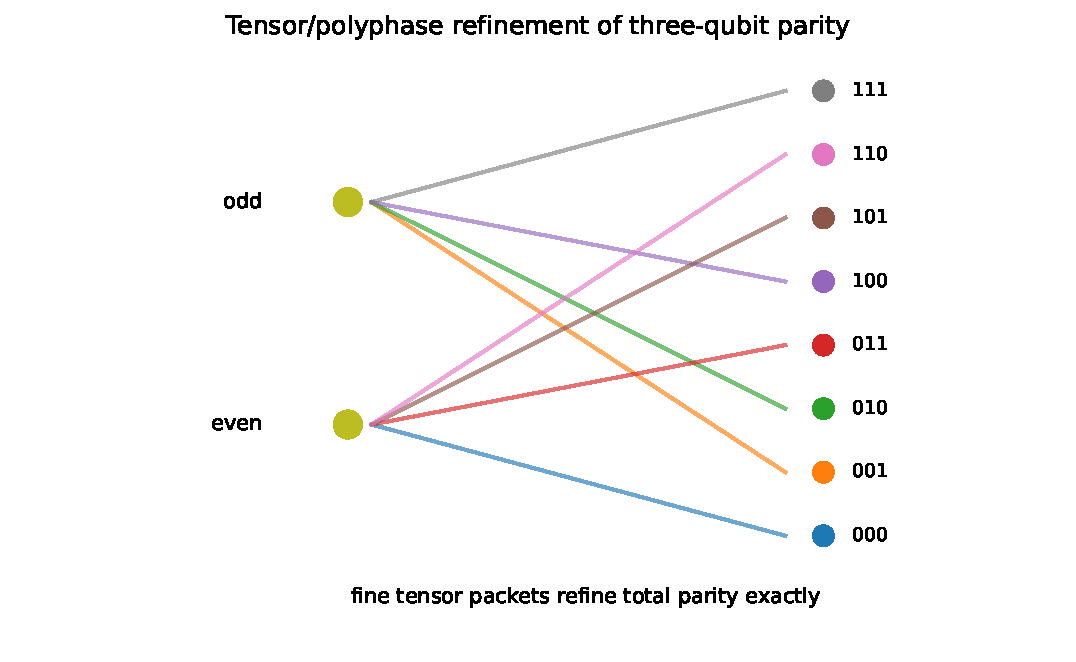
\includegraphics[width=0.86\textwidth]{10_tensor_parity_refinement.pdf}
\caption{The eight computational packets of three qubits refine the two total-parity packets exactly.}
\label{fig:tensor-refinement}
\end{figure}

\begin{certificate}[Exact parity refinement]
For three qubits, the local computational projectors were grouped by Hamming-weight parity. The resulting coarse projectors agreed with $(I\pm Z^{\otimes3})/2$ with residual $0$.
\end{certificate}

\section{Quantum circuits as packet paths}

Let
\[
U=U_mU_{m-1}\cdots U_1
\]
be a circuit and let $\{P_\alpha\}$ be a complete packet system.

\begin{theorem}[Exact circuit path expansion]
For source packet $\alpha_0$ and target packet $\alpha_m$,
\[
\boxed{
P_{\alpha_m}UP_{\alpha_0}
=
\sum_{\alpha_1,\ldots,\alpha_{m-1}}
P_{\alpha_m}U_mP_{\alpha_{m-1}}
\cdots
P_{\alpha_1}U_1P_{\alpha_0}.
}
\]
Summing over the source and target packets reconstructs the complete circuit operator.
\end{theorem}

\begin{proof}
Insert the identity resolution $I=\sum_\alpha P_\alpha$ between every adjacent pair of gates. Distributing the finite sums gives the path expansion. Summing the left and right boundary projectors reconstructs $U$.
\end{proof}

\begin{theorem}[Packetwise unitarity conservation]
If $U$ is unitary and $U_{\beta\alpha}=P_\beta UP_\alpha$, then
\[
\boxed{
\sum_\beta U_{\beta\alpha}^*U_{\beta\gamma}
=
\delta_{\alpha\gamma}P_\alpha.
}
\]
Similarly,
\[
\sum_\alpha U_{\beta\alpha}U_{\delta\alpha}^*
=
\delta_{\beta\delta}P_\beta.
\]
\end{theorem}

\begin{proof}
Using completeness and unitarity,
\[
\sum_\beta U_{\beta\alpha}^*U_{\beta\gamma}
=
P_\alpha U^*\left(\sum_\beta P_\beta\right)UP_\gamma
=
P_\alpha P_\gamma.
\]
The second identity is analogous.
\end{proof}

\begin{example}[Bell seed circuit]
Starting from $\ket{00}$,
\[
(H\otimes I)\ket{00}
=
\frac{\ket{00}+\ket{10}}{\sqrt2},
\]
and then
\[
\operatorname{CNOT}(H\otimes I)\ket{00}
=
\frac{\ket{00}+\ket{11}}{\sqrt2}.
\]
The parity packets show that the final state lies entirely in the even sector, while the intermediate circuit path passes through both even and odd addresses.
\end{example}

\begin{figure}[htbp]
\centering
\begin{minipage}[t]{0.48\textwidth}
\centering
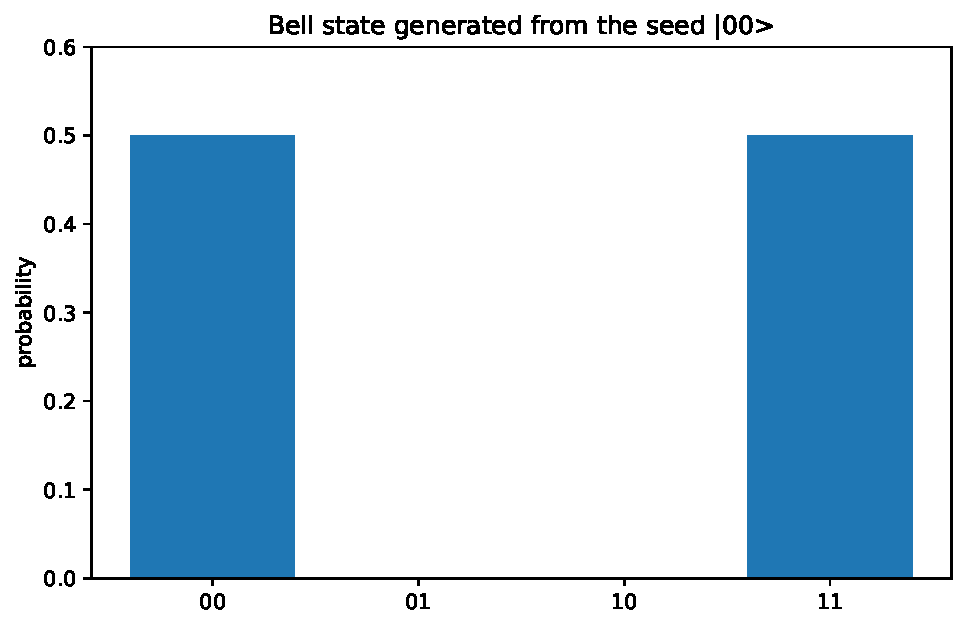
\includegraphics[width=\textwidth]{02_bell_seed_probabilities.pdf}
\captionof{figure}{The Bell state generated from the seed $\ket{00}$.}
\label{fig:bell}
\end{minipage}\hfill
\begin{minipage}[t]{0.48\textwidth}
\centering
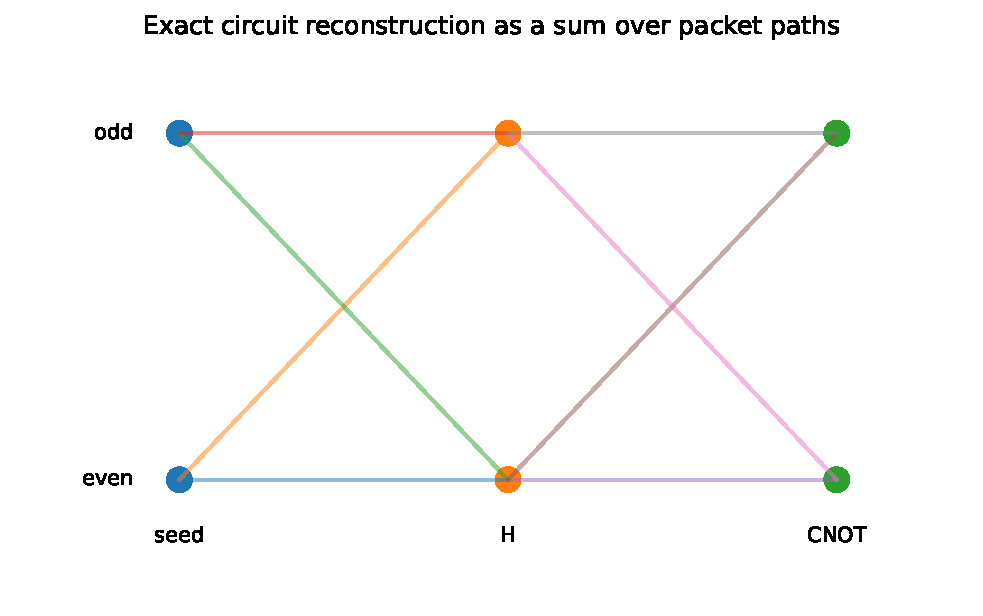
\includegraphics[width=\textwidth]{04_circuit_packet_paths.pdf}
\captionof{figure}{Circuit reconstruction as a sum over packet paths.}
\label{fig:circuit-paths}
\end{minipage}
\end{figure}

\begin{certificate}[Bell and path reconstruction]
The Bell-state residual and the complete parity-path reconstruction residual were both $0$ in the numerical implementation.
\end{certificate}

\section{Symmetry-resolved Hamiltonians and leakage}

Let $H=H^*$ and let $P$ be a packet projector. If $[H,P]=0$, then $P\cH$ is invariant under $e^{-itH}$.

\begin{theorem}[Exact symmetry packets]
If $[H,P_\alpha]=0$ for every packet, then
\[
H=\sum_\alpha P_\alpha HP_\alpha
\]
and
\[
e^{-itH}
=
\sum_\alpha P_\alpha e^{-itH}P_\alpha.
\]
No amplitude transfers between distinct packets.
\end{theorem}

\begin{proof}
The commutation relation gives $P_\beta HP_\alpha=0$ for $\beta\ne\alpha$. Every polynomial in $H$ has the same block form, and the finite-dimensional exponential is the norm limit of its polynomial series.
\end{proof}

For two qubits, consider
\[
H
=
JX\otimes X
+h(Z\otimes I+I\otimes Z).
\]
In the ordered even basis $\{\ket{00},\ket{11}\}$ and odd basis $\{\ket{01},\ket{10}\}$,
\[
H_{\mathrm{even}}
=
\begin{pmatrix}
2h&J\\
J&-2h
\end{pmatrix},
\qquad
H_{\mathrm{odd}}
=
\begin{pmatrix}
0&J\\
J&0
\end{pmatrix}.
\]
Therefore
\[
\Spec H_{\mathrm{even}}
=\{\pm\sqrt{4h^2+J^2}\},
\qquad
\Spec H_{\mathrm{odd}}=\{\pm J\}.
\]

\begin{figure}[htbp]
\centering
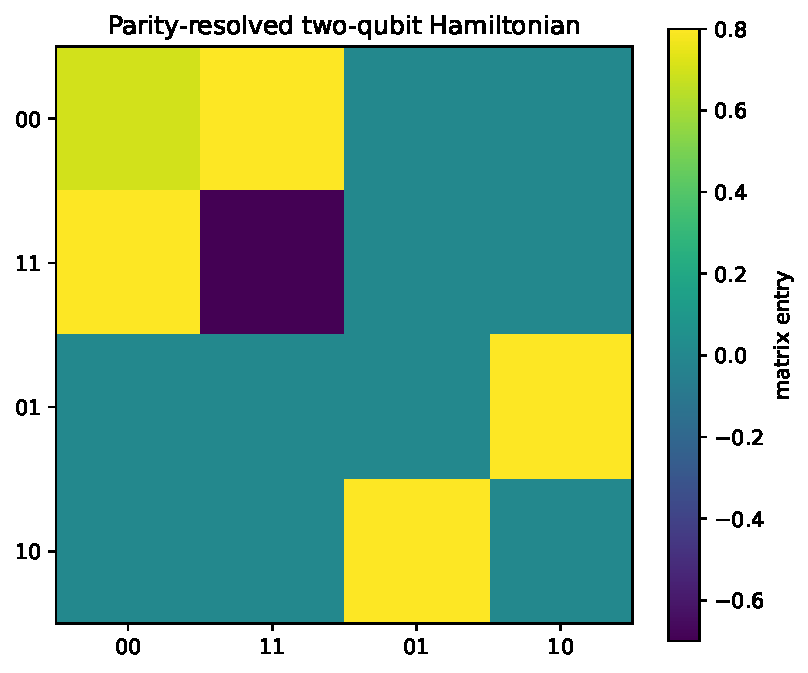
\includegraphics[width=0.66\textwidth]{03_parity_block_hamiltonian.pdf}
\caption{The parity-resolved Hamiltonian is exactly block diagonal after the even and odd basis vectors are grouped.}
\label{fig:parity-hamiltonian}
\end{figure}

\subsection{Leakage under broken symmetry}

Set $Q=I-P$.

\begin{theorem}[Commutator leakage bound]
For every self-adjoint $H$, orthogonal projector $P$, and real time $t$,
\[
\boxed{
\norm{Qe^{-itH}P}
\le
|t|\,\norm{[H,P]}.
}
\]
In particular, exact commutation gives zero leakage for all time.
\end{theorem}

\begin{proof}
Because $QP=0$,
\[
Qe^{-itH}P
=Q[e^{-itH},P]P.
\]
The Duhamel identity gives
\[
[e^{-itH},P]
=-i\int_0^t e^{-i(t-s)H}[H,P]e^{-isH}\,ds.
\]
Both unitary factors have norm one, so taking norms yields the bound.
\end{proof}

\begin{figure}[htbp]
\centering
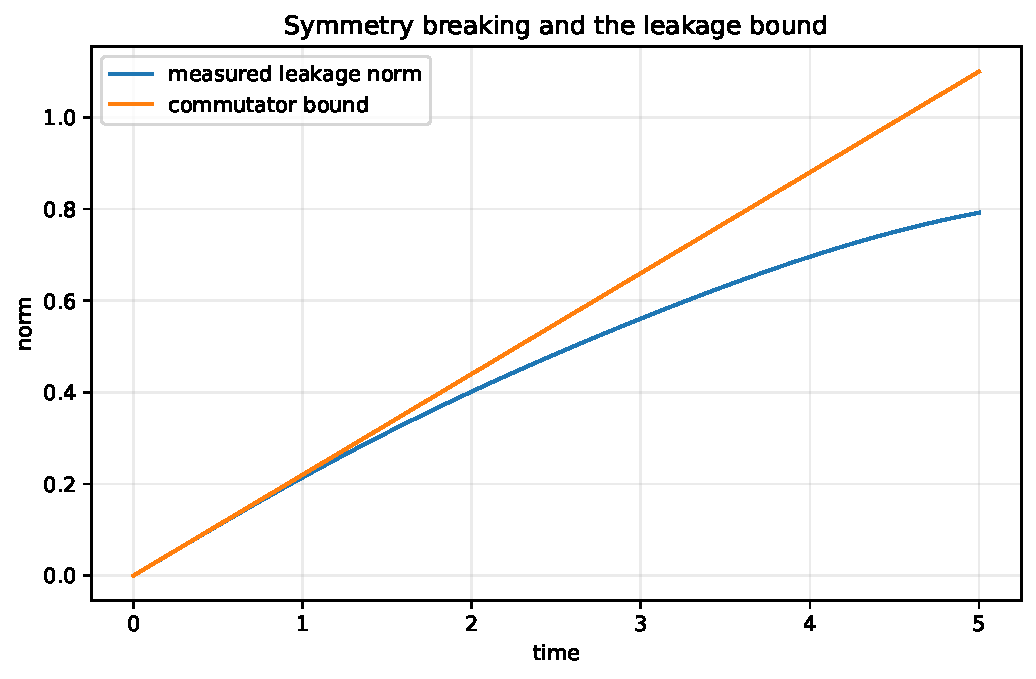
\includegraphics[width=0.78\textwidth]{05_leakage_bound.pdf}
\caption{A parity-breaking perturbation creates nonzero transfer between the packets, while the measured leakage remains below the commutator bound.}
\label{fig:leakage}
\end{figure}

\begin{certificate}[Symmetry and negative control]
For the parity-preserving Hamiltonian, the off-packet block norm and maximum measured leakage were both $0$. After adding a parity-breaking $X\otimes I$ perturbation, the maximum leakage was approximately $0.79196$, and the maximum violation of the proved bound was $0$.
\end{certificate}

\section{Moving packets, connections, and curvature}

\subsection{Moving quantum coordinates}

\begin{theorem}[Moving-frame Hamiltonian]
Let $U(t)$ be differentiable and unitary, and suppose
\[
i\dot\psi(t)=H(t)\psi(t).
\]
Writing
\[
\psi(t)=U(t)y(t)
\]
gives
\[
\boxed{
i\dot y(t)
=
\left(U(t)^*H(t)U(t)-iU(t)^*\dot U(t)\right)y(t).
}
\]
The connection term $-iU^*\dot U$ is Hermitian.
\end{theorem}

\begin{proof}
Differentiate $\psi=Uy$:
\[
i\dot U y+iU\dot y=HUy.
\]
Multiplying by $U^*$ gives the formula. Differentiating $U^*U=I$ shows $U^*\dot U$ is skew-Hermitian, so $-iU^*\dot U$ is Hermitian.
\end{proof}

\begin{figure}[htbp]
\centering
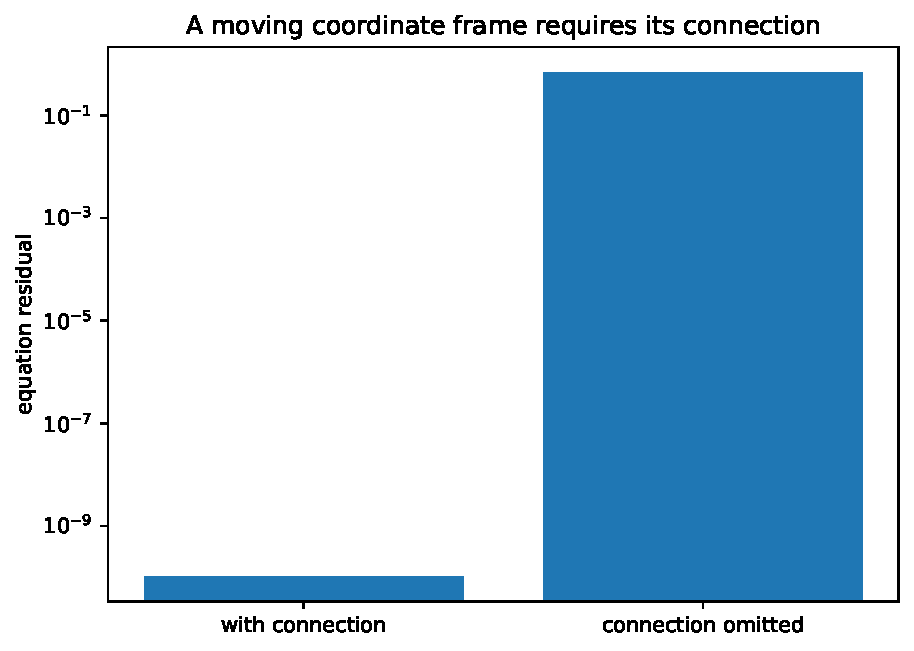
\includegraphics[width=0.70\textwidth]{08_moving_frame_connection.pdf}
\caption{The moving-frame equation closes to numerical precision only when the connection term is retained.}
\label{fig:moving-frame}
\end{figure}

\begin{certificate}[Moving-frame correction]
The complete moving-frame equation had residual $1.0645\times10^{-10}$, while omitting the connection produced residual $0.7000$.
\end{certificate}

\subsection{A canonical projector connection}

Let $P_1(t),\ldots,P_m(t)$ be differentiable orthogonal projectors satisfying
\[
P_aP_b=\delta_{ab}P_a,
\qquad
\sum_aP_a=I.
\]

\begin{theorem}[Canonical packet connection]
Define
\[
\boxed{
C(t)
=
\frac12\sum_a[\dot P_a(t),P_a(t)]
=
\sum_a\dot P_a(t)P_a(t).
}
\]
Then
\[
C(t)^*=-C(t)
\]
and
\[
\boxed{
[C(t),P_b(t)]=\dot P_b(t)
}
\]
for every packet $b$.
\end{theorem}

\begin{proof}
Differentiating $P_a^2=P_a$ gives
\[
\dot P_aP_a+P_a\dot P_a=\dot P_a.
\]
Summing over $a$ and using $\sum_a\dot P_a=0$ yields
\[
\sum_aP_a\dot P_a=-\sum_a\dot P_aP_a,
\]
which proves both displayed formulas for $C$ and its skew-Hermiticity.

For fixed $b$,
\[
CP_b=\dot P_bP_b.
\]
When $a\ne b$, differentiating $P_bP_a=0$ gives
\[
P_b\dot P_a=-\dot P_bP_a.
\]
Hence
\[
P_bC
=\sum_aP_b\dot P_aP_a
=-\dot P_b(I-P_b),
\]
and subtraction gives $[C,P_b]=\dot P_b$.
\end{proof}

The connection is the infinitesimal transport operator of the moving packet frame. It is determined by the packet family itself, without choosing a basis inside any packet.

\subsection{Projector curvature}

\begin{classical}[Projected connection]
For a smooth projector-valued map $P$ on a parameter manifold, the connection on the range bundle is $\nabla=P\,d$. Its curvature is
\[
\boxed{
F=P(dP\wedge dP)P.
}
\]
\end{classical}

\begin{proof}
For a section $s$ with $Ps=s$,
\[
\nabla^2s
=P\,d(P\,ds)
=P(dP)\wedge ds.
\]
Since $ds=d(Ps)=(dP)s+Pds$ and $P(dP)P=0$, the surviving term is
\[
P(dP\wedge dP)Ps.
\]
\end{proof}

For a rank-one projector, the scalar curvature density is
\[
\cF_{\mu\nu}
=-i\Tr\left(P[\partial_\mu P,\partial_\nu P]\right).
\]
On the Bloch sphere,
\[
P(\theta,\phi)
=
\frac12\left(I+\mathbf n(\theta,\phi)\cdot\boldsymbol\sigma\right),
\]
where
\[
\mathbf n=(\sin\theta\cos\phi,\sin\theta\sin\phi,\cos\theta).
\]
The Pauli multiplication law gives
\[
\boxed{
\cF_{\theta\phi}
=\frac12\sin\theta.
}
\]

\begin{figure}[htbp]
\centering
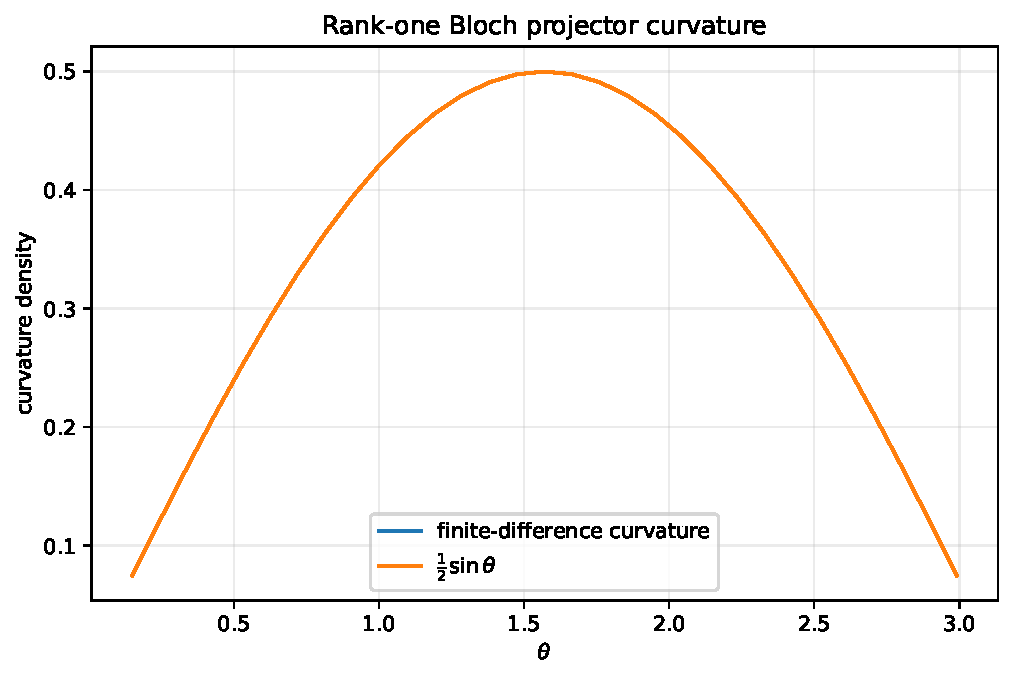
\includegraphics[width=0.76\textwidth]{09_bloch_curvature.pdf}
\caption{Finite-difference evaluation of the Bloch projector curvature against the exact density $\frac12\sin\theta$.}
\label{fig:bloch}
\end{figure}

\begin{certificate}[Geometric packet identities]
The canonical connection reconstructed every packet derivative with residual $0$. The maximum Bloch-curvature residual was $2.0803\times10^{-11}$.
\end{certificate}

\section{Measurements and quantum channels}

\subsection{Packet measurements}

Let $\rho$ be a density matrix and let $\{E_k\}$ be a POVM:
\[
E_k\ge0,
\qquad
\sum_kE_k=I.
\]
The outcome probabilities are
\[
p_k=\Tr(E_k\rho).
\]

\begin{theorem}[Block-diagonal measurement invariance]
Let $\{P_\alpha\}$ be a complete packet family, and suppose every measurement effect is packet diagonal:
\[
E_k=\sum_\alpha P_\alpha E_kP_\alpha.
\]
Define the packet-dephased state
\[
\cD_P(\rho)=\sum_\alpha P_\alpha\rho P_\alpha.
\]
Then
\[
\boxed{
\Tr(E_k\rho)
=
\Tr(E_k\cD_P(\rho))
}
\]
for every outcome $k$.
\end{theorem}

\begin{proof}
Insert the packet decomposition of $E_k$ and use cyclicity of the trace:
\[
\Tr(E_k\rho)
=
\sum_\alpha\Tr(P_\alpha E_kP_\alpha\rho)
=
\sum_\alpha\Tr(E_kP_\alpha\rho P_\alpha).
\]
\end{proof}

This theorem says exactly what coherence a declared measurement can and cannot see. Coherence between different packets is invisible to every packet-diagonal observable, while coherence inside a packet remains available.

\subsection{Kraus transfer}

\begin{classical}[Finite Kraus channel]
Let $K_1,\ldots,K_r$ satisfy
\[
\sum_aK_a^*K_a=I.
\]
Then
\[
\boxed{
\Phi(\rho)=\sum_aK_a\rho K_a^*
}
\]
is completely positive and trace preserving.
\end{classical}

\begin{proof}
Trace preservation follows from
\[
\Tr\Phi(\rho)
=\Tr\left(\rho\sum_aK_a^*K_a\right)
=\Tr\rho.
\]
For any auxiliary dimension and positive matrix $X$, each term
\[
(I\otimes K_a)X(I\otimes K_a)^*
\]
is positive, so their sum is positive. This is complete positivity.
\end{proof}

Packet superoperator blocks are defined by
\[
\Phi_{\alpha\beta;\gamma\delta}(X)
=
P_\alpha
\Phi(P_\gamma XP_\delta)
P_\beta.
\]
Summing all four packet indices reconstructs $\Phi(X)$ exactly.

For amplitude damping with parameter $\gamma$,
\[
K_0=
\begin{pmatrix}
1&0\\0&\sqrt{1-\gamma}
\end{pmatrix},
\qquad
K_1=
\begin{pmatrix}
0&\sqrt\gamma\\0&0
\end{pmatrix}.
\]
The excited state becomes
\[
\Phi(\ket1\bra1)
=
\gamma\ket0\bra0+(1-\gamma)\ket1\bra1.
\]

\begin{figure}[htbp]
\centering
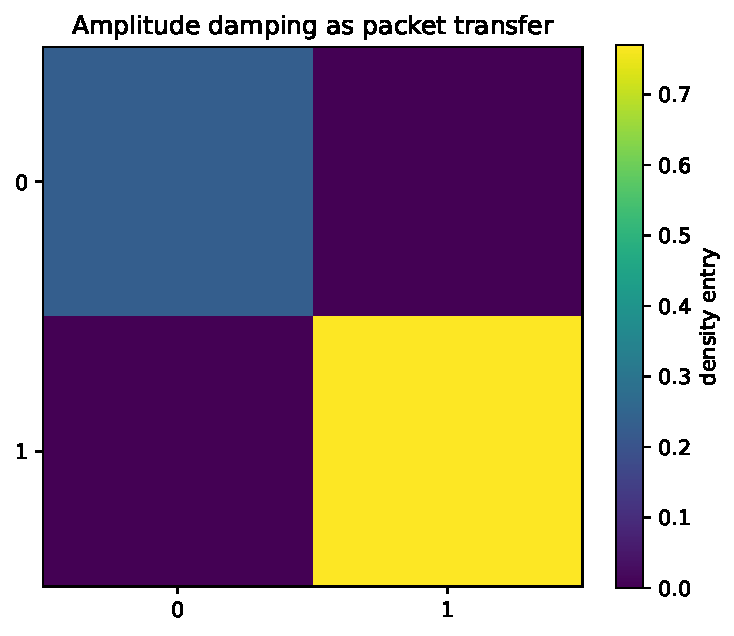
\includegraphics[width=0.56\textwidth]{16_amplitude_damping_channel.pdf}
\caption{Amplitude damping transfers population from the excited packet to the ground packet while preserving trace and positivity.}
\label{fig:damping}
\end{figure}

\begin{certificate}[Channel reconstruction]
For $\gamma=0.23$, the Kraus completeness and output-trace residuals were $0$. The computed output from $\ket1\bra1$ was $\diag(0.23,0.77)$. Packet dephasing changed no computational-basis measurement probability in the Bell-state test.
\end{certificate}

\section{Quantum error correction as obstruction-packet annihilation}

Let $P$ project onto a code space $\cC\subset\cH$, and let $E_1,\ldots,E_r$ be an error family. The operators
\[
P E_a^*E_bP
\]
are the code-level obstruction packets: if they retain logical-state information beyond one scalar multiple of $P$, the environment can distinguish logical states and exact correction is impossible.

\begin{classical}[Finite Knill--Laflamme criterion]
The error family is exactly correctable on $\cC$ if and only if there is a positive semidefinite matrix $(c_{ab})$ such that
\[
\boxed{
P E_a^*E_bP=c_{ab}P
}
\]
for every $a,b$.
\end{classical}

\begin{proof}
Assume first that a recovery corrects every error combination. Then inner products between corrupted code states cannot depend on the logical vector except through its original inner product. Polarization therefore gives
\[
\bra\psi E_a^*E_b\ket\phi
=c_{ab}\langle\psi,\phi\rangle
\]
for all $\psi,\phi\in\cC$, which is the displayed operator identity.

Conversely, diagonalize the positive matrix $c$ and replace the $E_a$ by the corresponding linear combinations $F_r$. Then
\[
PF_r^*F_sP=\lambda_r\delta_{rs}P.
\]
For $\lambda_r>0$, $F_r/\sqrt{\lambda_r}$ is an isometry from the code into an error subspace, and distinct error subspaces are orthogonal. A recovery first projects onto these syndrome packets and then applies the inverse isometry on each packet. This reconstructs every code state.
\end{proof}

For the three-qubit bit-flip code,
\[
\ket{0_L}=\ket{000},
\qquad
\ket{1_L}=\ket{111},
\]
and the error family is
\[
I,
\quad X\otimes I\otimes I,
\quad I\otimes X\otimes I,
\quad I\otimes I\otimes X.
\]
The four error images of the code are pairwise orthogonal two-dimensional syndrome packets whose projectors sum to the identity on the eight-dimensional Hilbert space.

\begin{figure}[htbp]
\centering
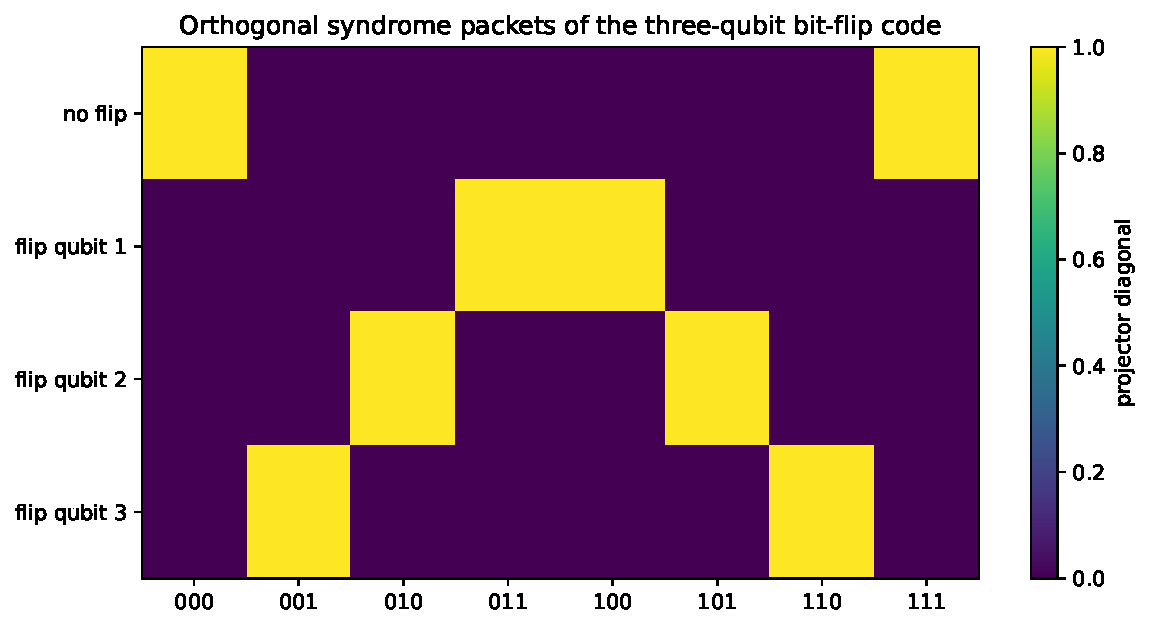
\includegraphics[width=0.88\textwidth]{19_error_correction_syndromes.pdf}
\caption{The four orthogonal syndrome packets of the three-qubit bit-flip code. Each packet identifies one correctable error without resolving the encoded logical state.}
\label{fig:error-correction}
\end{figure}

\begin{certificate}[Exact bit-flip correction]
The Knill--Laflamme residual and syndrome-completeness residual were both $0$. A mixed single-bit-flip channel applied to a nontrivial logical superposition was reversed with density-matrix residual $1.0385\times10^{-16}$.
\end{certificate}

\section{Exact effective dynamics}

\subsection{Schur--Feshbach reduction}

Let $P$ be a retained packet projector and $Q=I-P$. In packet coordinates,
\[
H=
\begin{pmatrix}
H_{PP}&H_{PQ}\\
H_{QP}&H_{QQ}
\end{pmatrix}.
\]

\begin{theorem}[Exact Feshbach resolvent]
If $z-H_{QQ}$ is invertible, define
\[
\boxed{
H_{\mathrm{eff}}(z)
=
H_{PP}
+H_{PQ}(z-H_{QQ})^{-1}H_{QP}.
}
\]
Then
\[
\boxed{
P(z-H)^{-1}P
=
\left(z-H_{\mathrm{eff}}(z)\right)^{-1}
}
\]
when both sides are written in an orthonormal basis of $P\cH$.
\end{theorem}

\begin{proof}
The block matrix $z-H$ has lower-right block $z-H_{QQ}$. Gaussian block elimination produces the Schur complement
\[
z-H_{PP}-H_{PQ}(z-H_{QQ})^{-1}H_{QP}.
\]
The upper-left block of the inverse is the inverse of this Schur complement, which is exactly the displayed operator.
\end{proof}

The self-energy
\[
\Sigma_P(z)
=H_{PQ}(z-H_{QQ})^{-1}H_{QP}
\]
contains the complete influence of the eliminated packet. Bare truncation drops $\Sigma_P(z)$ and is therefore exact only when the cross-packet coupling vanishes or the self-energy cancels for another stated reason.

\begin{figure}[htbp]
\centering
\begin{minipage}[t]{0.48\textwidth}
\centering
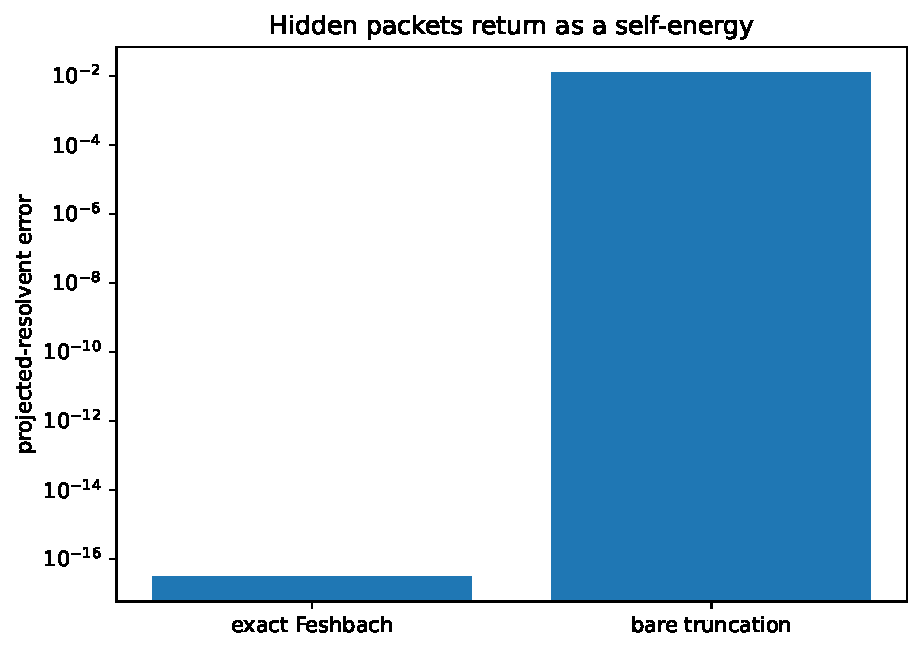
\includegraphics[width=\textwidth]{06_feshbach_vs_truncation.pdf}
\captionof{figure}{Exact Feshbach reduction versus bare truncation.}
\label{fig:feshbach}
\end{minipage}\hfill
\begin{minipage}[t]{0.48\textwidth}
\centering
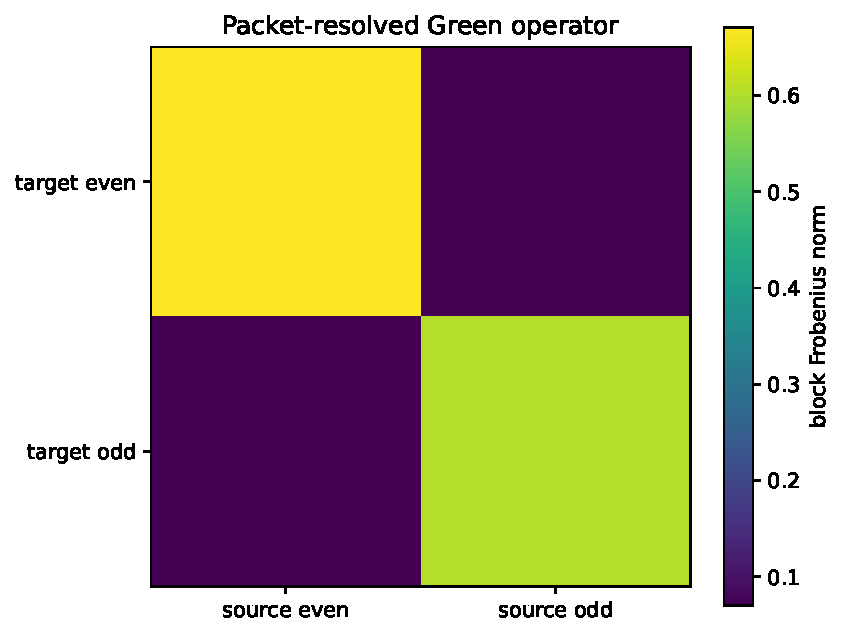
\includegraphics[width=\textwidth]{07_packet_green_blocks.pdf}
\captionof{figure}{Norms of packet Green-function blocks.}
\label{fig:green-blocks}
\end{minipage}
\end{figure}

\begin{certificate}[Effective resolvent]
For a random six-dimensional Hermitian test, the exact Feshbach residual was $3.2291\times10^{-17}$. The corresponding bare-truncation residual was $1.3091\times10^{-2}$.
\end{certificate}

\subsection{The hidden packet as memory}

Write $\psi=x+y$, with $x=P\psi$ and $y=Q\psi$. Then
\[
\begin{aligned}
i\dot x&=H_{PP}x+H_{PQ}y,\\
i\dot y&=H_{QP}x+H_{QQ}y.
\end{aligned}
\]
Solving the second equation gives
\[
y(t)
=e^{-itH_{QQ}}y(0)
-i\int_0^t e^{-i(t-s)H_{QQ}}H_{QP}x(s)\,ds.
\]
Substitution yields the exact Volterra equation
\[
\boxed{
\begin{aligned}
i\dot x(t)
={}&H_{PP}x(t)
+H_{PQ}e^{-itH_{QQ}}y(0)\\
&-i\int_0^t
K(t-s)x(s)\,ds,
\end{aligned}
}
\]
with memory kernel
\[
\boxed{
K(t)=H_{PQ}e^{-itH_{QQ}}H_{QP}.
}
\]
Thus hidden packets do not disappear. They become a frequency-dependent self-energy in resolvent coordinates and a causal memory kernel in time coordinates.

\section{Finite quantum geometry}

\subsection{A projector-resolved geometry}

At resolution $\ell$, define
\[
\boxed{
\mathfrak Q_\ell
=
\left(
\cA_\ell,
\cH_\ell,
D_\ell,
\{P_{\ell,\alpha}\},
E_\ell,
C_\ell,
\Pi_\ell^{\mathrm{phys}},
T_\ell
\right).
}
\]
The entries are an observable algebra, Hilbert space, geometric or Dirac-type operator, packet projectors, fine embedding, coarse reconstruction, physical constraint projector, and transfer operator.

A coherent refinement should satisfy
\[
C_\ell E_\ell=I
\]
and
\[
\boxed{
P_{\ell,\alpha}
=
C_\ell
\left(
\sum_{\beta\succ\alpha}P_{\ell+1,\beta}
\right)
E_\ell.
}
\]
For an operator $D$, define the refinement defect
\[
\Delta_\ell(D)
=C_\ell D_{\ell+1}E_\ell-D_\ell.
\]
Exact resolution independence is $\Delta_\ell(D)=0$. When exact equality is too strong, the correct continuum problem is to prove convergence of the resolvents and uniform control of the effective self-energies.

\begin{figure}[htbp]
\centering
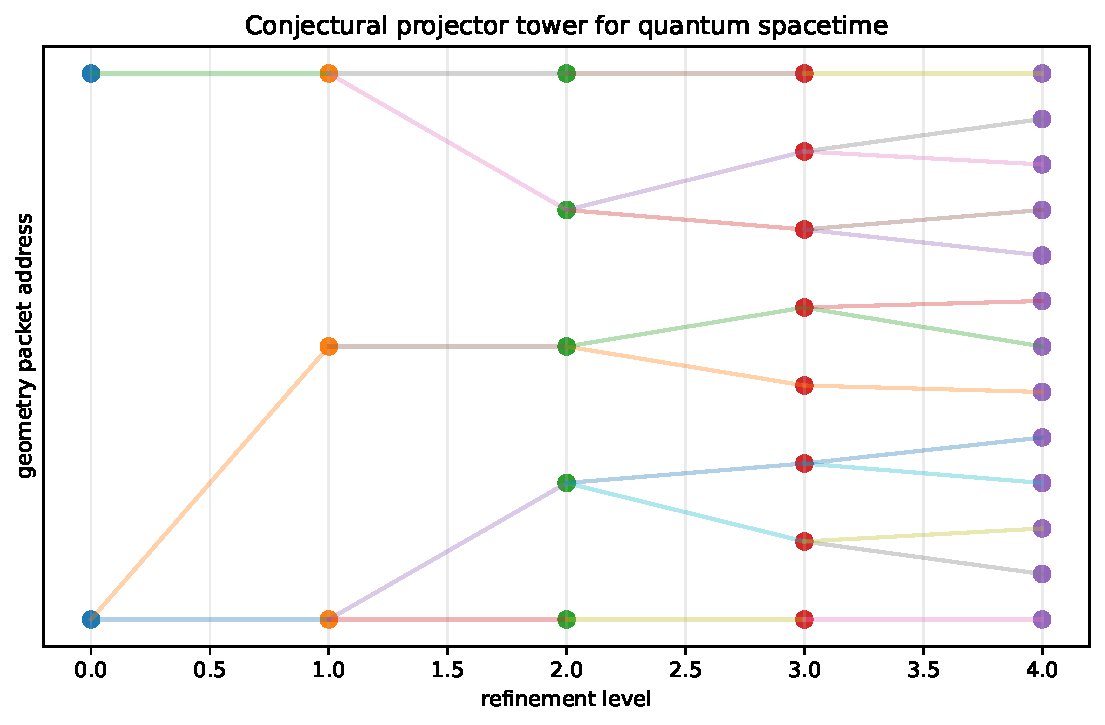
\includegraphics[width=0.84\textwidth]{17_quantum_spacetime_tower.pdf}
\caption{A conjectural nested packet tower for quantum geometry. The diagram is an organizational model; it is not a numerical reconstruction of physical spacetime.}
\label{fig:spacetime-tower}
\end{figure}

\subsection{Euclidean transfer}

\begin{theorem}[Finite Euclidean transfer]
For every finite Hermitian $H$ bounded below and every $\tau\ge0$,
\[
T(\tau)=e^{-\tau(H-E_0I)},
\qquad
E_0=\min\Spec H,
\]
is positive definite and satisfies
\[
\boxed{
T(\tau+\sigma)=T(\tau)T(\sigma).
}
\]
Its spectrum is contained in $(0,1]$.
\end{theorem}

\begin{proof}
Diagonalize $H=\sum_jE_jP_j$. Then
\[
T(\tau)=\sum_j e^{-\tau(E_j-E_0)}P_j.
\]
Every eigenvalue is positive and at most one. Multiplication adds the exponents, proving the semigroup law.
\end{proof}

The paper tests a controlled volume-state model
\[
H_{nn}=2\kappa+V(n),
\qquad
H_{n,n+1}=H_{n+1,n}=-\kappa,
\]
with a confining potential. This is a finite transfer-matrix test only. It is not derived from a gravitational path integral and is not evidence for a unique microscopic spacetime dynamics.

\begin{figure}[htbp]
\centering
\begin{minipage}[t]{0.48\textwidth}
\centering
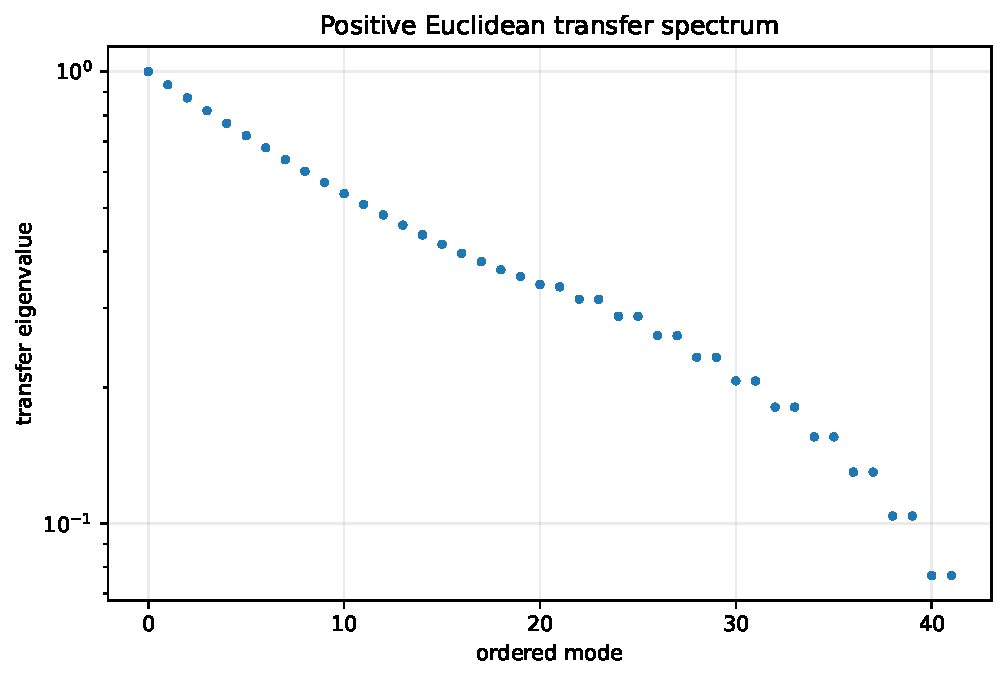
\includegraphics[width=\textwidth]{13_euclidean_transfer_spectrum.pdf}
\captionof{figure}{Positive spectrum of the Euclidean transfer operator.}
\label{fig:euclidean-spectrum}
\end{minipage}\hfill
\begin{minipage}[t]{0.48\textwidth}
\centering
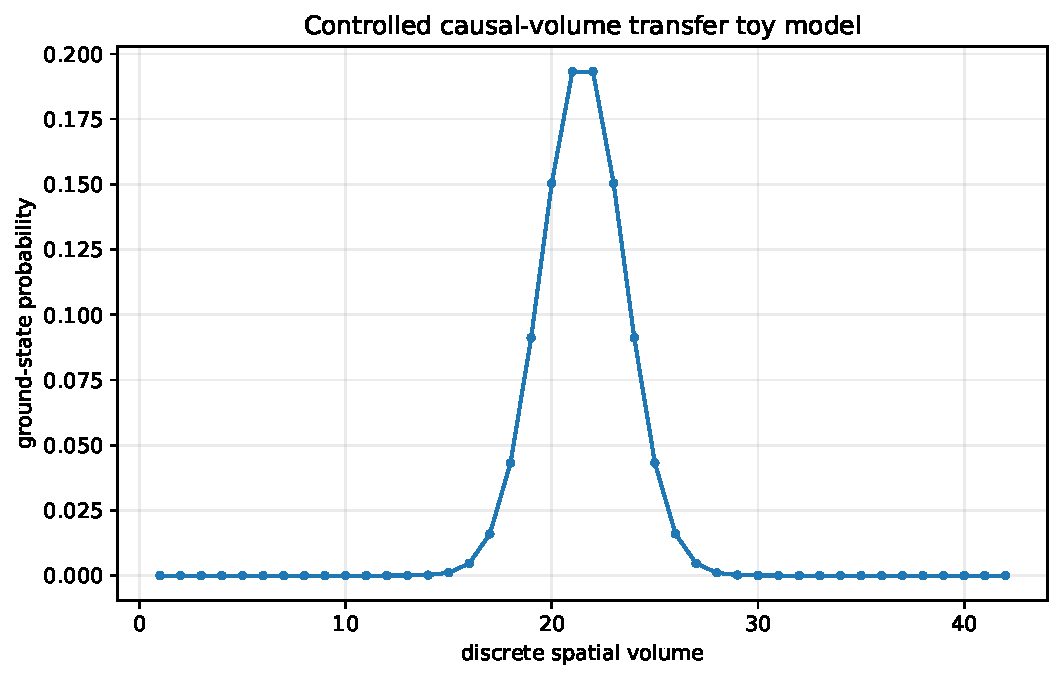
\includegraphics[width=\textwidth]{14_causal_volume_ground_state.pdf}
\captionof{figure}{Ground-state volume packet in the controlled toy model.}
\label{fig:volume-ground}
\end{minipage}
\end{figure}

\begin{figure}[htbp]
\centering
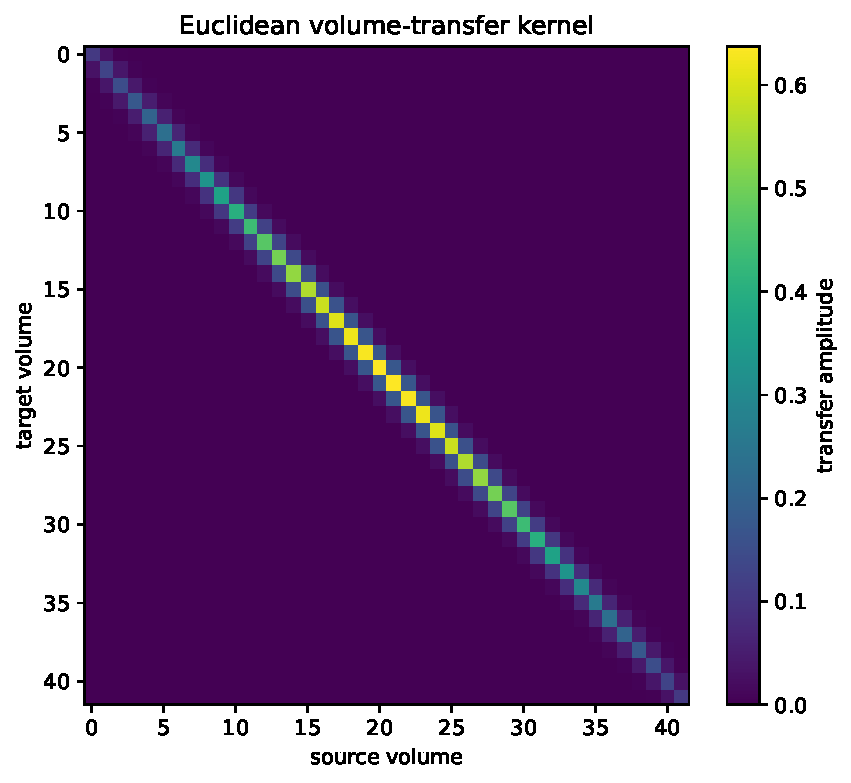
\includegraphics[width=0.68\textwidth]{15_causal_volume_transfer.pdf}
\caption{The finite Euclidean volume-transfer kernel. Positivity and semigroup composition are exact finite statements; its gravitational interpretation remains provisional.}
\label{fig:volume-transfer}
\end{figure}

\begin{certificate}[Finite transfer model]
The minimum transfer eigenvalue was $0.0767054$, the semigroup residual was $0$, and reconstruction from four volume-residue packets had residual $0$.
\end{certificate}

\section{Spectral dimension and continuum diagnostics}

Let $L\ge0$ be a finite Laplacian with eigenvalues $\lambda_j$. Define the normalized heat trace
\[
K(\tau)=\frac1N\sum_j e^{-\tau\lambda_j}
\]
and the scale-dependent spectral dimension
\[
\boxed{
d_s(\tau)
=-2\frac{d\log K(\tau)}{d\log\tau}.
}
\]
For a finite system, $d_s(\tau)$ is a diagnostic, not a topological invariant. At very small diffusion time it sees the ultraviolet lattice, and at very large time it collapses toward the zero mode. A geometric dimension can only be inferred from a stable intermediate window and a controlled refinement limit.

\subsection{The circle dispersion bound}

For a periodic grid with spacing $h$,
\[
\lambda_{k,h}
=
\frac4{h^2}\sin^2\left(\frac{kh}{2}\right).
\]

\begin{theorem}[Low-mode second-order bound]
If $0\le kh/2\le1$, then
\[
\boxed{
0\le k^2-\lambda_{k,h}
\le
\frac{k^4h^2}{12}.
}
\]
\end{theorem}

\begin{proof}
Set $x=kh/2$. Since $\sin x\le x$, the error is nonnegative. On $[0,1]$,
\[
\sin x\ge x-\frac{x^3}{6}.
\]
Therefore
\[
\sin^2x
\ge
\left(x-\frac{x^3}{6}\right)^2
\ge
x^2-\frac{x^4}{3}.
\]
Hence
\[
x^2-\sin^2x\le\frac{x^4}{3}.
\]
Multiplication by $4/h^2$ gives the result.
\end{proof}

\begin{figure}[htbp]
\centering
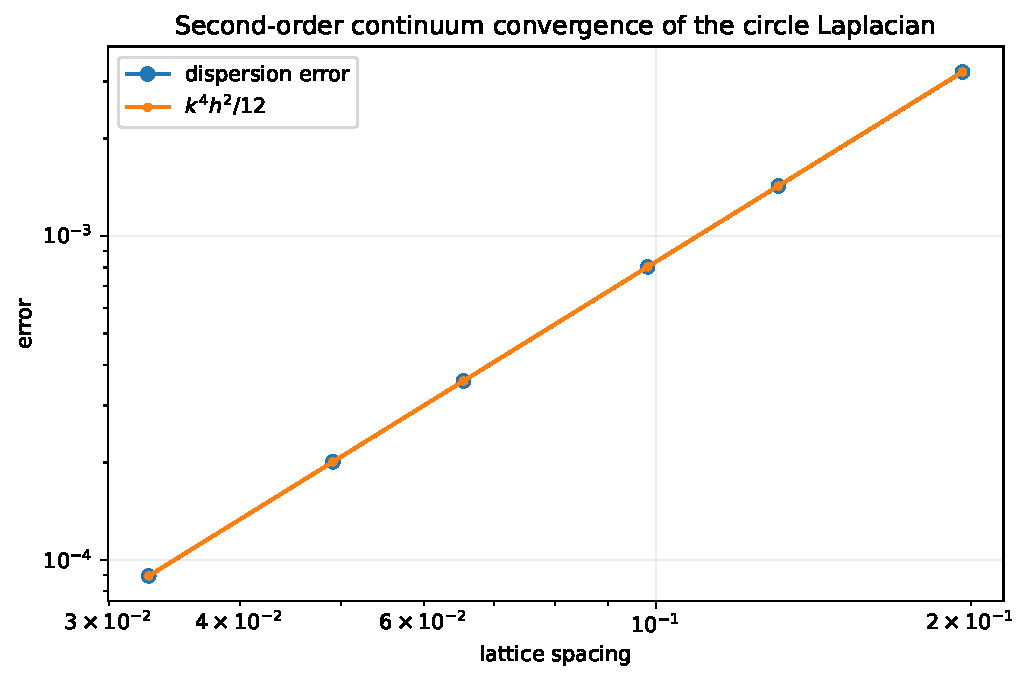
\includegraphics[width=0.76\textwidth]{11_circle_low_mode_convergence.pdf}
\caption{The first nonzero circle mode converges at second order and remains below the proved dispersion bound.}
\label{fig:circle-convergence}
\end{figure}

\begin{certificate}[Continuum dispersion]
The observed convergence order was $1.99936$. The maximum error-minus-bound value was negative, so no tested mode violated the theorem.
\end{certificate}

\subsection{One- and two-dimensional plateaus}

\begin{figure}[htbp]
\centering
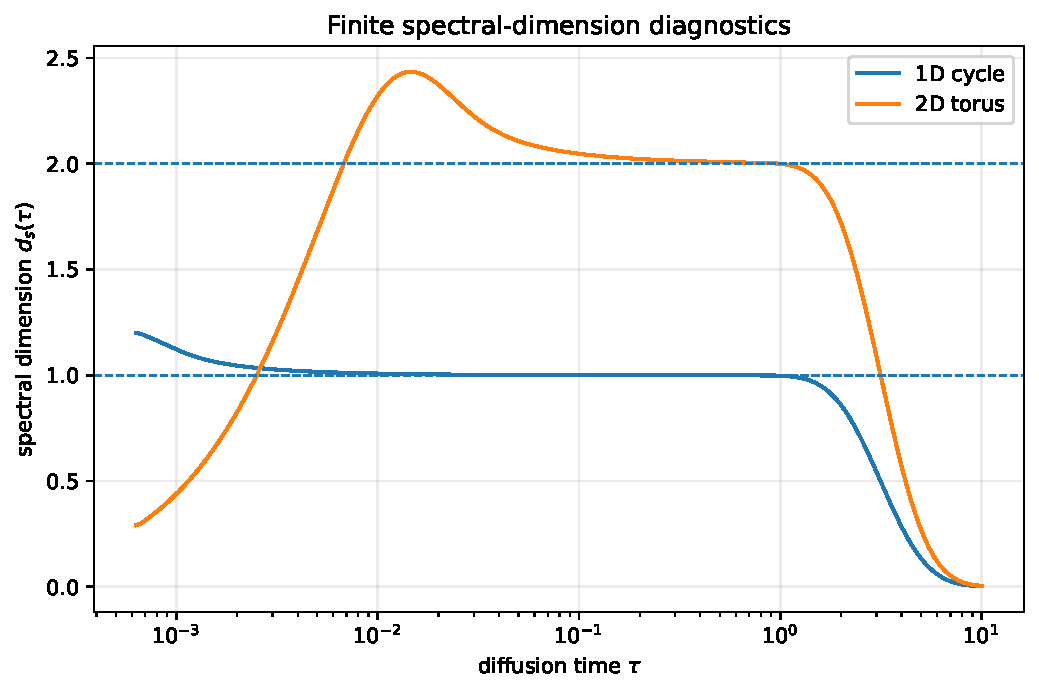
\includegraphics[width=0.80\textwidth]{12_spectral_dimension.pdf}
\caption{Intermediate spectral-dimension windows for a finite cycle and a finite two-dimensional torus. The ultraviolet and infrared departures are finite-size effects, not additional dimensions.}
\label{fig:spectral-dimension}
\end{figure}

\begin{certificate}[Spectral dimension]
The median intermediate plateaus were
\[
d_s^{(1)}=1.00062,
\qquad
d_s^{(2)}=2.03781.
\]
These tests recover the expected dimensions of the chosen finite geometries; they do not select a physical quantum-spacetime theory.
\end{certificate}

\section{Constraint packets and the quantum-spacetime boundary}

Let $\widehat C_A$ be quantum constraints and let $\Pi^{\mathrm{phys}}$ project onto their common kernel. If the classical constraint algebra has structure coefficients $f_{AB}^{\ \ C}$, define the anomaly operator
\[
\boxed{
\mathfrak A_{AB}
=
[\widehat C_A,\widehat C_B]
-i\sum_C f_{AB}^{\ \ C}\widehat C_C.
}
\]
Its physical packet is
\[
\Pi^{\mathrm{phys}}\mathfrak A_{AB}\Pi^{\mathrm{phys}}.
\]
A nonzero physical anomaly packet is an explicit obstruction to exact constraint closure.

\begin{conjecture}[Anomaly-free refinement]
There exists a coherent quantum-geometric packet tower for which
\[
\Pi^{\mathrm{phys}}_\ell
\mathfrak A^{(\ell)}_{AB}
\Pi^{\mathrm{phys}}_\ell=0
\]
at every level and the physical projectors reconstruct compatibly under refinement.
\end{conjecture}

\begin{conjecture}[Uniform Feshbach control]
For the same tower, the self-energies produced by exact elimination of fine packets admit bounds uniform in the cutoff and volume on a common spectral domain. These bounds yield a strong-resolvent continuum limit.
\end{conjecture}

\begin{conjecture}[Lorentzian reconstruction]
The Euclidean packet theory satisfies a positivity or reconstruction principle strong enough to produce a Lorentzian Hilbert space with causal propagation and positive physical norm.
\end{conjecture}

\begin{conjecture}[Einstein infrared limit]
There exist semiclassical packet states $\Psi_{g,\ell}$ such that the effective action converges to
\[
\frac1{16\pi G}
\int\sqrt{-g}\,(R-2\Lambda)\,d^4x
\]
with controlled higher-order corrections.
\end{conjecture}

\begin{conjecture}[Massless spin-two sector]
The continuum two-point function possesses a positive transverse-traceless massless spin-two pole, while all unphysical packet sectors are removed by the constraints.
\end{conjecture}

These conjectures are logically independent of the exact finite identities. Exact packet reconstruction is a kinematic and computational advantage; it does not determine the physical action, prove continuum existence, or guarantee the general-relativistic limit.

\begin{figure}[htbp]
\centering
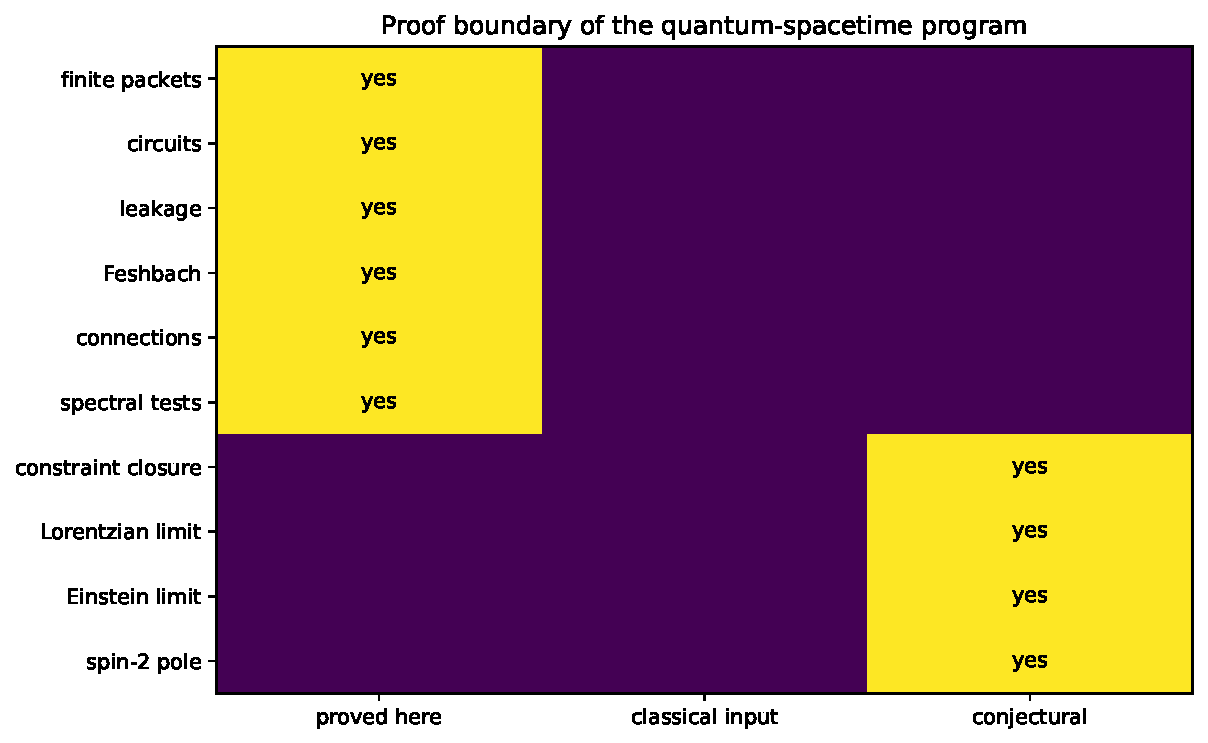
\includegraphics[width=0.86\textwidth]{18_proof_boundary.pdf}
\caption{The proof boundary. Finite packet, circuit, leakage, Feshbach, connection, and spectral identities are established here. Constraint closure and the physical continuum claims remain conjectural.}
\label{fig:proof-boundary}
\end{figure}

\section{Numerical certificates}

All experiments in this paper were run on CPU. No GPU result is claimed.

\begin{table}[htbp]
\centering
\caption{Representative finite numerical certificates.}
\label{tab:certificates}
\begin{tabular}{L{0.64\textwidth}r}
\toprule
Certificate & Value\\
\midrule
Bell-state residual & $0$\\
Three-qubit seed-orbit rank & $8/8$\\
Parity off-block norm & $0$\\
Circuit path reconstruction residual & $0$\\
Exact-symmetry maximum leakage & $0$\\
Maximum leakage-bound violation & $0$\\
Feshbach projected-resolvent residual & $3.2291\times10^{-17}$\\
Bare-truncation projected-resolvent residual & $1.3091\times10^{-2}$\\
Moving-frame residual with connection & $1.0645\times10^{-10}$\\
Moving-frame residual without connection & $7.0000\times10^{-1}$\\
Canonical packet-connection residual & $0$\\
Bloch-curvature residual & $2.0803\times10^{-11}$\\
Kraus completeness residual & $0$\\
Output trace residual & $0$\\
Knill--Laflamme residual & $0$\\
Bit-flip recovery residual & $1.0385\times10^{-16}$\\
Tensor parity-refinement residual & $0$\\
Circle low-mode convergence order & $1.99936$\\
One-dimensional spectral plateau & $1.00062$\\
Two-dimensional spectral plateau & $2.03781$\\
Minimum Euclidean-transfer eigenvalue & $0.0767054$\\
Transfer semigroup residual & $0$\\
Volume-packet reconstruction residual & $0$\\
\bottomrule
\end{tabular}
\end{table}

The complete automated suite passed
\[
\boxed{22/22\text{ tests}.}
\]
The results are stored in machine-readable JSON and CSV form. Every figure in the paper is generated by the accompanying Python package.

\section{Software realization}

The companion implementation is organized by mathematical responsibility:

\begin{longtable}{L{0.28\textwidth}L{0.64\textwidth}}
\toprule
Module & Responsibility\\
\midrule
\endfirsthead
\toprule
Module & Responsibility\\
\midrule
\endhead
\texttt{basic.py} & basis states, Pauli gates, tensor embeddings, packet blocks, cyclic and multi-generator reachability\\
\texttt{symmetry.py} & finite cyclic projectors, parity packets, tensor refinement, sector populations\\
\texttt{circuits.py} & circuit composition and exact packet-path reconstruction\\
\texttt{dynamics.py} & unitary evolution, leakage bounds, Feshbach reduction, moving frames, canonical connections, Bloch curvature\\
\texttt{channels.py} & Kraus maps, measurements, and packet dephasing\\
\texttt{codes.py} & bit-flip code, syndrome packets, Knill--Laflamme certificate, and recovery\\
\texttt{geometry.py} & cycle and torus spectra, heat trace, spectral dimension, dispersion bounds, and Euclidean volume transfer\\
\texttt{experiments.py} & deterministic numerical certificate suite\\
\texttt{visuals.py} & all code-generated paper figures\\
\bottomrule
\end{longtable}

The implementation is deliberately finite-dimensional. Infinite-dimensional limits require separate domain, compactness, convergence, positivity, and renormalization arguments and are not inferred from the finite code.

\section{Conclusion}

The quantum realization of the seed calculus can now be stated precisely. A primitive state is addressed by a declared operator grammar; symmetry projectors split the state and every operator into exact packets; circuit products become sums over packet paths; Hamiltonian symmetry and its controlled breaking are visible as diagonal blocks and leakage; moving packets carry a canonical connection and curvature; channels, measurements, and error-correction conditions admit exact packet formulations; and eliminated sectors return through self-energy and memory rather than disappearing.

The finite theory therefore provides a coherent language for
\[
\boxed{
\begin{gathered}
\text{seed reachability}
+
\text{symmetry resolution}
+
\text{circuit paths}\\
+
\text{effective dynamics}
+
\text{geometric transport}
+
\text{constraint diagnostics}
\end{gathered}
}
\]
What it does not yet provide is the physical continuum theorem. The next decisive results would be anomaly-free refinement, uniform effective-operator control, Lorentzian reconstruction, the Einstein infrared limit, and a positive massless spin-two sector. Those requirements are explicit enough to be tested and too substantial to be replaced by finite numerical resemblance.

\end{document}
